\documentclass{article}
\usepackage{ctex}
\usepackage{amsmath}
\usepackage{graphicx}
\usepackage{float}
\usepackage{booktabs}
\usepackage{geometry}
\usepackage{listings}
\usepackage{xcolor}
\usepackage{titling}
\geometry{a4paper, margin=2.5cm}

% 让目录标题居中
\renewcommand{\contentsname}{\centerline{\Large\bfseries 目录}}

% 配置listings包,优化中文显示
\lstset{
    basicstyle=\small\ttfamily,
    keywordstyle=\color{blue},
    commentstyle=\color{green!60!black},
    stringstyle=\color{red},
    numbers=left,
    numberstyle=\tiny\color{gray},
    numbersep=5pt,
    breaklines=true,
    showspaces=false,
    showstringspaces=false,
    frame=single,
    tabsize=4,
    captionpos=b,
    backgroundcolor=\color{yellow!10}
}

\title{\Large\textbf{数值分析实验报告:插值方法比较}}
\author{\large 姓名:李忠鹏 \\ \large 学号:230980121}
\date{\large 2025年5月6日}

% 自定义封面
\renewcommand{\maketitle}{
  \begin{titlepage}
    \begin{center}
      \vspace*{2cm}
      
      {\Huge\bfseries 数值分析实验报告 \\[0.5cm]}
      {\LARGE\bfseries 插值方法比较 \\[2cm]}
      
      \begin{tabular}{rl}
        \Large\textbf{姓名:} & \Large\textbf{李忠鹏} \\[0.5cm]
        \Large\textbf{学号:} & \Large\textbf{230980121} \\[2cm]
      \end{tabular}
      
      \vfill
      
      {\Large\bfseries 2025年5月6日}
    \end{center}
  \end{titlepage}
}

\begin{document}

\maketitle

\tableofcontents
\clearpage

\section{问题描述}
本实验旨在比较两种不同的插值方法对平方根函数的近似效果。给定如下数据点:

\begin{table}[H]
\centering
\begin{tabular}{|c|ccccccccc|}
\hline
$x$ & 0 & 1 & 4 & 9 & 16 & 25 & 36 & 49 & 64 \\
\hline
$y$ & 0 & 1 & 2 & 3 & 4 & 5 & 6 & 7 & 8 \\
\hline
\end{tabular}
\caption{数据点(实际对应$y=\sqrt{x}$)}
\end{table}

实验要求:
\begin{enumerate}
    \item 用这9个点作8次多项式插值$L_8(x)$。
    \item 用三次样条(第一边界条件)程序求$S(x)$。
    \item 分析在区间$[0,64]$上,哪个插值更精确;在区间$[0,1]$上,两种插值哪个更精确。
\end{enumerate}

\section{理论基础}

\subsection{拉格朗日插值法}
拉格朗日插值法是一种多项式插值方法,用于构造一个$n$次多项式通过$n+1$个给定数据点。对于给定的数据点$(x_i, y_i)$,$i=0,1,\ldots,n$,拉格朗日插值多项式为:

\begin{equation}
L_n(x) = \sum_{i=0}^{n} y_i \cdot l_i(x)
\end{equation}

其中$l_i(x)$为拉格朗日基函数:

\begin{equation}
l_i(x) = \prod_{j=0,j\neq i}^{n} \frac{x-x_j}{x_i-x_j}
\end{equation}

每个基函数$l_i(x)$满足$l_i(x_i)=1$和$l_i(x_j)=0$(当$i\neq j$时)。

\subsection{三次样条插值法}
三次样条插值通过构造分段三次多项式来连接相邻数据点,保证曲线通过所有数据点,并且在节点处具有一阶和二阶导数的连续性。对于区间$[x_i,x_{i+1}]$上的三次多项式片段$S_i(x)$,其形式为:

\begin{equation}
S_i(x) = a_i + b_i(x-x_i) + c_i(x-x_i)^2 + d_i(x-x_i)^3
\end{equation}

第一边界条件指定在边界点处的二阶导数为0(自然边界条件)。

\section{代码实现}

\subsection{拉格朗日插值实现}
拉格朗日插值算法的核心实现如下:

\begin{verbatim}
def lagrange_interpolation(x_data, y_data):
    n = len(x_data)
    
    def lagrange_function(x):
        result = 0
        for i in range(n):
            Ln_value = y_data[i]
            for j in range(n):
                if i != j:
                    Ln_value *= (x - x_data[j]) / (x_data[i] - x_data[j])
            result += Ln_value
        return result
        
    return lagrange_function
\end{verbatim}

\subsection{三次样条插值实现}
三次样条插值使用了SciPy库中的CubicSpline函数:

\begin{verbatim}
from scipy.interpolate import CubicSpline
S = CubicSpline(x_data, y_data, bc_type='natural')
\end{verbatim}

其中\texttt{bc\_type='natural'}指定了自然边界条件(边界处的二阶导数为0)。

\section{结果分析}

\subsection{区间$[0,64]$上的插值效果}

图\ref{fig:lagrange_0_64}和图\ref{fig:spline_0_64}展示了两种插值方法在$[0,64]$区间上的效果对比。

\begin{figure}[H]
\centering
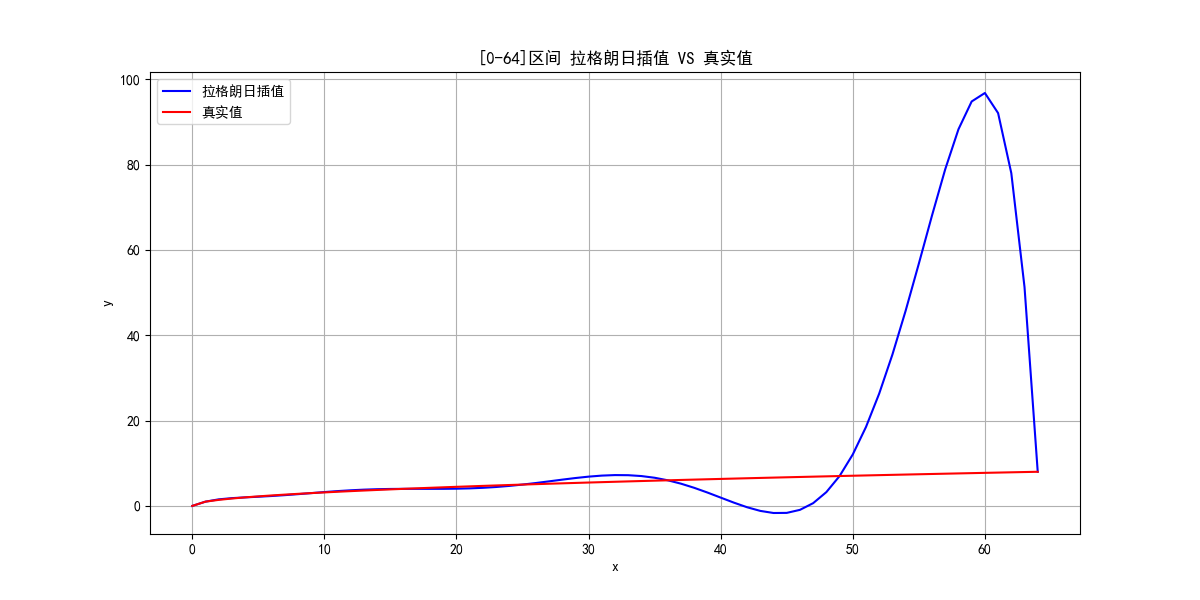
\includegraphics[width=0.9\textwidth]{./verify_results/lagrange/lagrange_interpolation_0_64.png}
\caption{拉格朗日插值在$[0,64]$区间上与真实函数的对比}
\label{fig:lagrange_0_64}
\end{figure}

\begin{figure}[H]
\centering
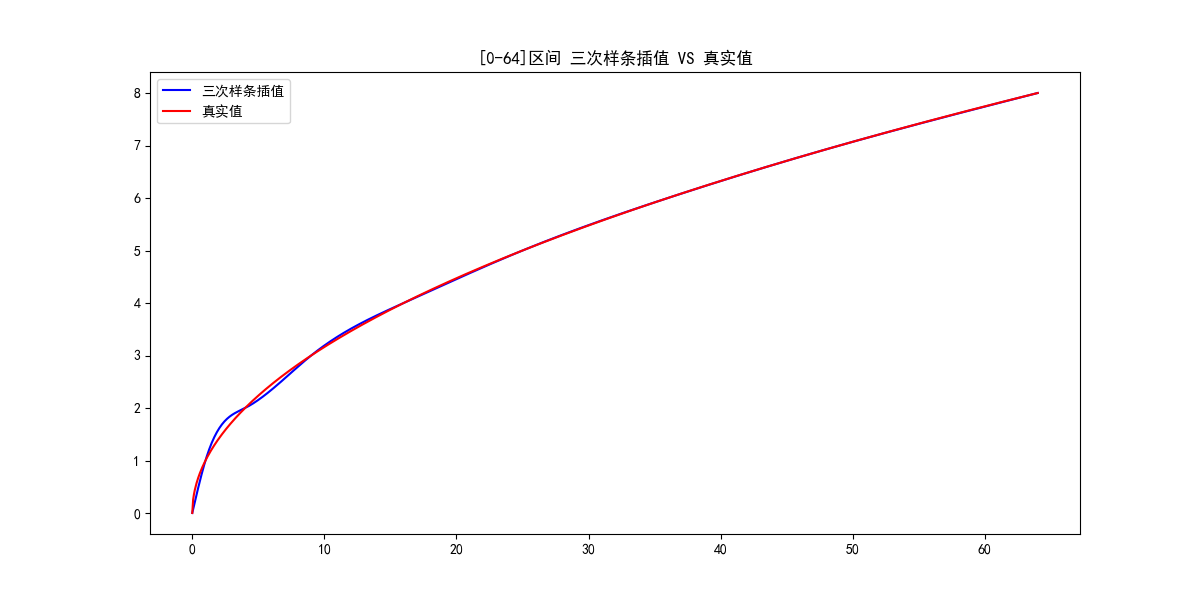
\includegraphics[width=0.9\textwidth]{./verify_results/CubicSpline/CubicSpline_0_64.png}
\caption{三次样条插值在$[0,64]$区间上与真实函数的对比}
\label{fig:spline_0_64}
\end{figure}

从图\ref{fig:lagrange_0_64}可以看出,拉格朗日8次多项式插值虽然通过了所有数据点,但在整个区间上出现了明显的震荡现象。而图\ref{fig:spline_0_64}显示,三次样条插值提供了更加平滑的曲线,与真实的平方根函数几乎完全重合。

\subsection{区间$[0,1]$上的插值效果}

图\ref{fig:lagrange_0_1}和图\ref{fig:spline_0_1}展示了两种方法在$[0,1]$区间上的效果。

\begin{figure}[H]
\centering
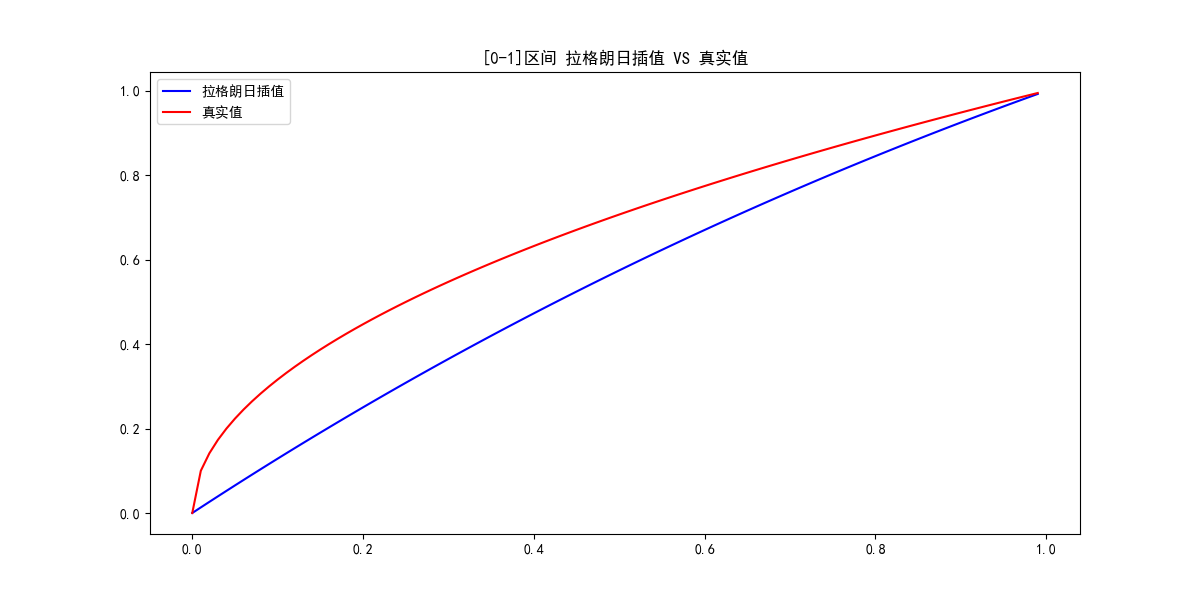
\includegraphics[width=0.9\textwidth]{./verify_results/lagrange/lagrange_interpolation_0_1.png}
\caption{拉格朗日插值在$[0,1]$区间上与真实函数的对比}
\label{fig:lagrange_0_1}
\end{figure}

\begin{figure}[H]
\centering
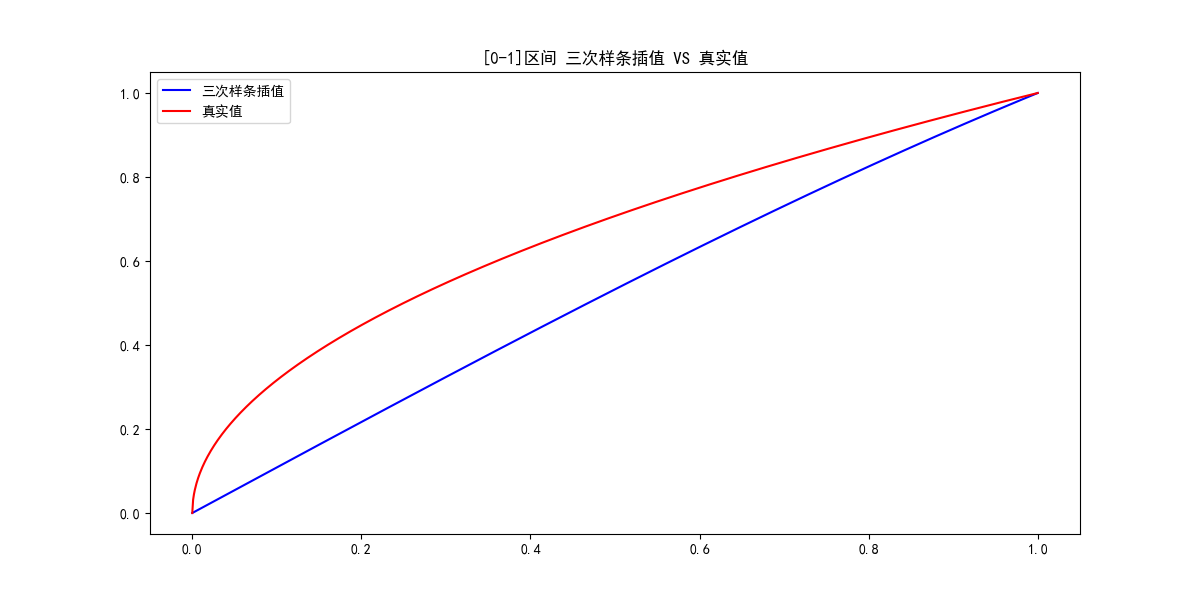
\includegraphics[width=0.9\textwidth]{./verify_results/CubicSpline/CubicSpline_0_1.png}
\caption{三次样条插值在$[0,1]$区间上与真实函数的对比}
\label{fig:spline_0_1}
\end{figure}

在区间$[0,1]$上,两种插值方法的表现相似,与真实函数都有良好的拟合。这主要是因为这个区间内只有两个数据点$(0,0)$和$(1,1)$,两种方法都能很好地插值这两个点。

\section{结论}

基于python跑出的结果和matplotlib画出的图像,可以得出以下结论:

\begin{enumerate}
    \item 在区间$[0,64]$上,三次样条插值明显优于拉格朗日插值。拉格朗日插值虽然通过所有数据点,但在数据点之间出现了明显的震荡(龙格现象),而三次样条插值保持了良好的平滑性,更接近真实函数。
    
    \item 在区间$[0,1]$上,两种插值方法的精确度相近。这主要是因为该区间内只有两个数据点,且函数在此区间内变化较为平缓。
\end{enumerate}

对于平方根函数的插值问题,三次样条插值法展现出了更好的整体性能,特别是在处理较大区间时能有效避免高次多项式插值的龙格现象,提供更加平滑和准确的近似结果。

\end{document}
